% Options for packages loaded elsewhere
\PassOptionsToPackage{unicode}{hyperref}
\PassOptionsToPackage{hyphens}{url}
%
\documentclass[
  12pt,
]{article}
\usepackage{amsmath,amssymb}
\usepackage{lmodern}
\usepackage{iftex}
\ifPDFTeX
  \usepackage[T1]{fontenc}
  \usepackage[utf8]{inputenc}
  \usepackage{textcomp} % provide euro and other symbols
\else % if luatex or xetex
  \usepackage{unicode-math}
  \defaultfontfeatures{Scale=MatchLowercase}
  \defaultfontfeatures[\rmfamily]{Ligatures=TeX,Scale=1}
\fi
% Use upquote if available, for straight quotes in verbatim environments
\IfFileExists{upquote.sty}{\usepackage{upquote}}{}
\IfFileExists{microtype.sty}{% use microtype if available
  \usepackage[]{microtype}
  \UseMicrotypeSet[protrusion]{basicmath} % disable protrusion for tt fonts
}{}
\makeatletter
\@ifundefined{KOMAClassName}{% if non-KOMA class
  \IfFileExists{parskip.sty}{%
    \usepackage{parskip}
  }{% else
    \setlength{\parindent}{0pt}
    \setlength{\parskip}{6pt plus 2pt minus 1pt}}
}{% if KOMA class
  \KOMAoptions{parskip=half}}
\makeatother
\usepackage{xcolor}
\IfFileExists{xurl.sty}{\usepackage{xurl}}{} % add URL line breaks if available
\IfFileExists{bookmark.sty}{\usepackage{bookmark}}{\usepackage{hyperref}}
\hypersetup{
  pdftitle={How reliable are inferences from state-space age-structured assessment models?},
  pdfauthor={Timothy J. Miller1, Britten, Brooks, Fay, Legault, Stock,},
  hidelinks,
  pdfcreator={LaTeX via pandoc}}
\urlstyle{same} % disable monospaced font for URLs
\usepackage[margin=1in]{geometry}
\usepackage{graphicx}
\makeatletter
\def\maxwidth{\ifdim\Gin@nat@width>\linewidth\linewidth\else\Gin@nat@width\fi}
\def\maxheight{\ifdim\Gin@nat@height>\textheight\textheight\else\Gin@nat@height\fi}
\makeatother
% Scale images if necessary, so that they will not overflow the page
% margins by default, and it is still possible to overwrite the defaults
% using explicit options in \includegraphics[width, height, ...]{}
\setkeys{Gin}{width=\maxwidth,height=\maxheight,keepaspectratio}
% Set default figure placement to htbp
\makeatletter
\def\fps@figure{htbp}
\makeatother
\setlength{\emergencystretch}{3em} % prevent overfull lines
\providecommand{\tightlist}{%
  \setlength{\itemsep}{0pt}\setlength{\parskip}{0pt}}
\setcounter{secnumdepth}{5}
\newlength{\cslhangindent}
\setlength{\cslhangindent}{1.5em}
\newlength{\csllabelwidth}
\setlength{\csllabelwidth}{3em}
\newlength{\cslentryspacingunit} % times entry-spacing
\setlength{\cslentryspacingunit}{\parskip}
\newenvironment{CSLReferences}[2] % #1 hanging-ident, #2 entry spacing
 {% don't indent paragraphs
  \setlength{\parindent}{0pt}
  % turn on hanging indent if param 1 is 1
  \ifodd #1
  \let\oldpar\par
  \def\par{\hangindent=\cslhangindent\oldpar}
  \fi
  % set entry spacing
  \setlength{\parskip}{#2\cslentryspacingunit}
 }%
 {}
\usepackage{calc}
\newcommand{\CSLBlock}[1]{#1\hfill\break}
\newcommand{\CSLLeftMargin}[1]{\parbox[t]{\csllabelwidth}{#1}}
\newcommand{\CSLRightInline}[1]{\parbox[t]{\linewidth - \csllabelwidth}{#1}\break}
\newcommand{\CSLIndent}[1]{\hspace{\cslhangindent}#1}
\usepackage{url}
\usepackage{setspace}
%\singlespacing
%\onehalfspacing
\doublespacing
\usepackage{lineno}
\linenumbers
\usepackage[belowskip=0pt,aboveskip=0pt]{caption}
\usepackage{relsize}
\newcommand{\afrb}{Alaska Fishery Research Bulletin\xspace}
\newcommand{\ajms}{African Journal of Marine Science\xspace}
\newcommand{\amb}{Advances in Marine Biology\xspace}
\newcommand{\bms}{Bulletin of Marine Science\xspace}
\newcommand{\bjssf}{Bulletin of the Japanese Society of Scientific Fisheries\xspace}
\newcommand{\cb}{Conservation Biology\xspace}
\newcommand{\cjfas}{Canadian Journal of Fisheries and Aquatic Sciences\xspace}
\newcommand{\ea}{Ecological Applications\xspace}
\newcommand{\eer}{Evolutionary Ecology Research\xspace}
\newcommand{\elet}{Ecology Letters\xspace}
\newcommand{\emod}{Ecological Modelling\xspace}
\newcommand{\ebf}{Environmental Biology of Fishes\xspace}
\newcommand{\ff}{Fish and Fisheries\xspace}
\newcommand{\fo}{Fisheries Oceanography\xspace}
\newcommand{\fr}{Fisheries Research\xspace}
\newcommand{\fb}{Fishery Bulletin\xspace}
\newcommand{\ijms}{ICES Journal of Marine Science\xspace}
\newcommand{\iccat}{Collective Volume of Scientific Papers ICCAT\xspace}
\newcommand{\jae}{Journal of Animal Ecology\xspace}
\newcommand{\jai}{Journal of Applied Ichthyology\xspace}
\newcommand{\jdc}{Journal Du Conseil International Pour L'exploration De La Mer\xspace}
\newcommand{\jdcp}{Journal Du Conseil Permanent International Pour L'exploration De La Mer\xspace}
\newcommand{\jembe}{Journal of Experimental Marine Biology and Ecology\xspace}
\newcommand{\jfb}{Journal of Fish Biology\xspace}
\newcommand{\jsr}{Journal of Sea Research\xspace}
\newcommand{\jtb}{Journal of Theoretical Biology\xspace}
\newcommand{\jfrbc}{Journal of the Fisheries Research Board of Canada\xspace}
\newcommand{\jnwafs}{Journal of Northwest Atlantic Fisheries Science\xspace}
\newcommand{\mcf}{Marine and Coastal Fisheries: Dynamics, Management, and Ecosystem Science\xspace}
\newcommand{\mb}{Marine Biology\xspace}
\newcommand{\meps}{Marine Ecology Progress Series\xspace}
\newcommand{\mfr}{Marine Fisheries Review\xspace}
\newcommand{\mpb}{Marine Pollution Bulletin\xspace}
\newcommand{\najfm}{North American Journal of Fisheries Management\xspace}
\newcommand{\nzjmfr}{New Zealand Journal of Marine and Freshwater Research\xspace}
\newcommand{\pnas}{Proceedings of the National Academy of Sciences USA\xspace}
\newcommand{\rpvrciemm}{Rapports et Proc\`es-Verbaux des R\'eunions. Conseil Internationale pour l'Exploration de la Mer\xspace}
\newcommand{\rpvrcpiemm}{Rapports et Proc\`es-Verbaux des R\'eunions. Conseil Permanent Internationale pour l'Exploration de la Mer\xspace}
\newcommand{\rfbf}{Reviews in Fish Biology and Fisheries\xspace}
\newcommand{\sajms}{South African Journal of Marine Science\xspace}
\newcommand{\tafs}{Transactions of the American Fisheries Society\xspace}

\newcommand{\anzjs}{Australian \& New Zealand Journal of Statistics\xspace}
\newcommand{\as}{Applied Statistics\xspace}
\newcommand{\csda}{Computational Statistics \& Data Analysis\xspace}
\newcommand{\ees}{Environmental and Ecological Statistics\xspace}
\newcommand{\jas}{Journal of Applied Statistics\xspace}
\newcommand{\jabes}{Journal of Agricultural, Biological, and Environmental Statistics\xspace}
\newcommand{\jasa}{Journal of the American Statistical Association\xspace}
\newcommand{\jrssb}{Journal of the Royal Statistical Society. Series B\xspace}
\newcommand{\sm}{Statistics in Medicine}

\usepackage{xspace}
\usepackage{bm}
\usepackage{caption,graphics}
\usepackage{graphicx}
\usepackage{makecell}
\renewcommand\figurename{Fig.}
\captionsetup{labelsep=period, singlelinecheck=false}
\newcommand{\changesize}[1]{\fontsize{#1pt}{#1pt}\selectfont}
\renewcommand{\arraystretch}{1.5}
\renewcommand\theadfont{}
\usepackage{booktabs}
\usepackage{longtable}
\usepackage{array}
\usepackage{multirow}
\usepackage{wrapfig}
\usepackage{float}
\usepackage{colortbl}
\usepackage{pdflscape}
\usepackage{tabu}
\usepackage{threeparttable}
\usepackage{threeparttablex}
\usepackage[normalem]{ulem}
\usepackage{makecell}
\usepackage{xcolor}
\ifLuaTeX
  \usepackage{selnolig}  % disable illegal ligatures
\fi
\usepackage[]{natbib}
\bibliographystyle{cjfas2.bst}

\title{How reliable are inferences from state-space age-structured
assessment models?}
\author{Timothy J. Miller\textsuperscript{1}, Britten, Brooks, Fay,
Legault, Stock,}
\date{}

\begin{document}
\maketitle

\(^1\)corresponding author:
\href{mailto:timothy.j.miller@noaa.gov}{\nolinkurl{timothy.j.miller@noaa.gov}},
Northeast Fisheries Science Center, Woods Hole Laboratory, 166 Water
Street, Woods Hole, MA 02543 USA\\

\pagebreak

\hypertarget{abstract}{%
\subsection*{Abstract}\label{abstract}}
\addcontentsline{toc}{subsection}{Abstract}

\hypertarget{keywords}{%
\subsubsection*{Keywords}\label{keywords}}
\addcontentsline{toc}{subsubsection}{Keywords}

\pagebreak

\hypertarget{introduction}{%
\section{Introduction}\label{introduction}}

Application of state-space models in fisheries stock assessment and
management has expanded dramatically within ICES, Canada and the
Northeast US \citep{nielsenberg14,cadigan16,stockmiller21}.

Much is known about the reliability of state-space models that are
linear or Gaussian \citep{aeberhardetal18}, but applications in
fisheries management are nonlinear and typically include multiple types
of observations with varying distributional assumptions. We know
relatively little about the statistical reliability of such models.
Also, there is a wide range of potential random effects structures in
assessment models and we know little about the ability of information
criteria to distinguish among such alternative structures.

But those studies focus primarily on Gaussian linear models. review
literature on reliability of hidden/latent process models. Primarily in
other fields.

\hypertarget{methods}{%
\section{Methods}\label{methods}}

Used the WHAM package \citep[][commit 77bbd94]{stockmiller21} (Miller
and Stock 2020). This packages has also been used to configure operating
and estimating models for closed loop simulations evaluating index-based
assessment methods \citep{legaultetalinpress}.

We completed a simulation study with a number of operating models that
can be categorized based on where random effects are assumed: abundance
at age, natural mortality, fleet selectivity, or index catchability. For
each operating model assumptions about variance of process errors and
observations are required and the values we used were based on a review
of the range of estimates from recent applications of WHAM in management
of stocks of haddock, butterfish, and American plaice in the NE US.

We simulated 100 data sets for each operating model. For each simulated
data from each operating model we fit a set of estimating models.

Y estimating models fit to each

\hypertarget{operating-models}{%
\subsection{Operating models}\label{operating-models}}

common to all:\\
ages = 1 to 10+, M maturity

marginal standard deviations for random effects are defined in tables of
operating models.

\hypertarget{population}{%
\subsubsection{Population}\label{population}}

There are 10 age classes: ages 1 to 10+.

Spawning was assumed to occur 1/4 of the way through the year.

Natural mortality rate was assumed 0.2 when it was constant and the mean
of the time series process for operating models with M random effects.
maturity a50 = 2.89, slope = 0.88

Weight at age was generated with a LVB growth \[
L_a = L_{\infty}\left(1 - e^{-k(a - t_0)}\right)
\] where \(t_0 = 0\), \(L_\infty = 85\), and \(k = 0.3\), and a L-W
relationship such that \[
W_a = \theta_1 L_a^{\theta_2}
\] where \(\theta_1 = e^{-12.1}\) and \(\theta_2 = 3.2\).

We assumed a Beverton-Holt stock recruit function with constant
pre-recruit mortality parameters for all operating models. All
post-recruit productivity components are constant in the NAA and survey
catchability process error operating models. Therefore steepness and
unfished recruitment are also constant over the time period for those
operating models (Miller and Brooks 2021). We specified unfished
recruitment = \(R_0 = e^{10}\) and \(F_{\text{MSY}} = F_{40} = 0.348\)
equated to a steepness of 0.69 and \(\alpha=0.60\) and
\(\beta = 2.4 \times 10^{-5}\) for the \[
N_{1,y} = \frac{\alpha \text{SSB}_{y-1}}{1 + \beta \text{SSB}_{y-1}} 
\] Beverton-Holt parameterization.

The magnitude of the overfishing assumptions is based on average
estimates of overfishing for NE groundfish stocks from Wiedenmann et
al.~(20XX). Legault et al.~(2023) also used similar approaches to
defining fishing mortality histories for operating models.

Initial population was configured at the equilibrium distribution
fishing at either \(F = 2.5\times F_{\text{MSY}}\) or
\(F = F_{\text{MSY}}\) for the two alternative fishing histories. That
is for a deterministic model, the age composition would not change over
time when the fishing mortality was constant at the respective level.

For operating models with time-varying random effects for M, steepness
is not constant, but we used the same alpha and beta parameters as other
operating models this equates to a steepness and R0 at the mean of the
time series process for M. For operating models with time-varying random
effects for fishery selectivity, Fmsy is also not constant however we
use the same F history as other operating models which corresponds to
Fmsy at the mean selectivity parameters.

\hypertarget{fleets}{%
\subsubsection{Fleets}\label{fleets}}

We assumed a single fleet operating year round for catch observations
with logistic selectivity for the fleet with \(a_{50} = 5\) and slope =
1. This selectivity is was used to define \(F_{\text{MSY}}\) for the
Beverton-Holt stock recruitment parameters above. We assumed a
logistic-normal distribution for the age-composition observations for
the fleet.

\hypertarget{fishing-histories}{%
\subsubsection{Fishing histories}\label{fishing-histories}}

All operating models assumed one of two different fishing histories. One
: Fishing mortality is equal to Fmsy (0.348) for the whole 40 year
period. Two : Fishing mortality is 2.5 times Fmsy for the first 20 years
then changes to Fmsy for the last 20 years.

\hypertarget{indices}{%
\subsubsection{Indices}\label{indices}}

Two time series of surveys are assumed and observed in numbers rather
than biomass for the entire 40 year period with one occurring in the
spring (0.25 way through the year) and one in the fall (0.75 way through
the year). Actually we have it currently configured that both occur 0.5
way through the year. Catchability of both surveys are assumed to be
0.1. We assumed logistic selectivity for both indices with
\(a_{50} = 5\) and slope = 1. We assumed a logistic-normal distribution
for the age-composition observations.

\hypertarget{observation-uncertainty}{%
\subsubsection{Observation Uncertainty}\label{observation-uncertainty}}

Standard deviation for log-aggregate catch was 0.1. There were two
levels of observation error variance for indices and age composition for
both indices and fleet catch. A low uncertainty specification assumed
standard deviation of both series of log-aggregate index observations
was 0.1 and the standard deviation of the logistic-normal for age
composition observations was 0.3 In the high uncertainty specification
the standard deviation for log-aggregate indices was 0.4 and that for
the age composition observations was 1.5.

\hypertarget{operating-models-with-random-effects-on-numbers-at-age}{%
\subsubsection{Operating models with random effects on numbers at
age}\label{operating-models-with-random-effects-on-numbers-at-age}}

24 operating models, 16 Sel re operating models and 16 q re operating
models. Table of process error assumptions

\hypertarget{operating-models-with-random-effects-on-natural-mortality}{%
\subsubsection{Operating models with random effects on natural
mortality}\label{operating-models-with-random-effects-on-natural-mortality}}

16 operating models Table of process error assumptions

NOTE: inv\_trans\_rho function in set\_M.R is mis-defined. Will affect
correlation parameters assigned in operating models?

\hypertarget{operating-models-with-random-effects-on-fleet-selectivity}{%
\subsubsection{Operating models with random effects on fleet
selectivity}\label{operating-models-with-random-effects-on-fleet-selectivity}}

16 operating models Table of process error assumptions

\hypertarget{operating-models-with-random-effects-on-index-catchability}{%
\subsubsection{Operating models with random effects on index
catchability}\label{operating-models-with-random-effects-on-index-catchability}}

16 operating models Table of process error assumptions

\hypertarget{estimating-models}{%
\subsection{Estimating models}\label{estimating-models}}

32 estimating models Table of estimating models

1-20 fit to each NAA RE operating model 5-24 fit to each M RE operating
model 5-20,25-28 to each sel RE operating model 5-20, 29-32 to each q RE
operating model

SR estimation or not

Make plot of S-R curve, Fmsy = F40 Initial values for BH parameters are
the true values. Initial values for mean R model = true R0.

M estimation or not

NAA\_re Random effects on Recruitment only or random effects on
recruitment and transitions among older numbers at age.

M\_re Random effects on Recruitment only, M constant across age .

sel\_re Random effects on Recruitment only, fleet logistic selectivity
RE model?

q\_re Random effects on Recruitment only, one survey catchability RE
model?

Simulations were all carried out on the University of Massachussetts
Green High-Performance Computing Cluster. Code for completing the
simulations and summarization of results can be found at
github.com/timjmiller/SSRTWG/Project\_0. We used the wham package
version 1.X.X (commit XXXXX).

\hypertarget{results}{%
\section{Results}\label{results}}

Do each of these by type of operating model (Naa, M, sel, q) Convergence
performance

AIC performance

SR estimation? M estimation?

Bias, Mean Square error

Certain basic parameters (stock-recruit pars, M, variance parameters)
SSB, F, R

\clearpage

\hypertarget{numbers-at-age-operating-models}{%
\subsection{Numbers at age operating
models}\label{numbers-at-age-operating-models}}

\hypertarget{estimating-models-include-alternative-random-effects-options-naa-m-sel-q}{%
\subsubsection{Estimating models include alternative random effects
options: NAA, M, sel,
q}\label{estimating-models-include-alternative-random-effects-options-naa-m-sel-q}}

\clearpage

\begin{table}
\caption{NAA operating models, estimating models all assume a B-H stock recruit relationship and M is fixed at the true value.}
{\begin{center}
\begin{tabular}{rrrrrrrrr}
\hline\hline
\multicolumn{1}{c}{$\sigma_R$}&\multicolumn{1}{c}{$\sigma_N$}&\multicolumn{1}{c}{F-history}&\multicolumn{1}{c}{Obs Error}&\multicolumn{1}{c}{R only}&\multicolumn{1}{c}{NAA}&\multicolumn{1}{c}{M}&\multicolumn{1}{c}{Sel}&\multicolumn{1}{c}{q}\tabularnewline
\hline
$0.5$&$$&H-MSY&L&$98$&$  0$&$0$&$0$&$2$\tabularnewline
$1.5$&$$&H-MSY&L&$97$&$  0$&$0$&$0$&$3$\tabularnewline
$0.5$&$0.25$&H-MSY&L&$ 0$&$100$&$0$&$0$&$0$\tabularnewline
$1.5$&$0.25$&H-MSY&L&$ 0$&$ 99$&$1$&$0$&$0$\tabularnewline
$0.5$&$0.50$&H-MSY&L&$ 0$&$100$&$0$&$0$&$0$\tabularnewline
$1.5$&$0.50$&H-MSY&L&$ 0$&$ 99$&$1$&$0$&$0$\tabularnewline
$0.5$&$$&MSY&L&$97$&$  0$&$0$&$1$&$2$\tabularnewline
$1.5$&$$&MSY&L&$95$&$  0$&$0$&$1$&$4$\tabularnewline
$0.5$&$0.25$&MSY&L&$ 0$&$100$&$0$&$0$&$0$\tabularnewline
$1.5$&$0.25$&MSY&L&$ 0$&$100$&$0$&$0$&$0$\tabularnewline
$0.5$&$0.50$&MSY&L&$ 0$&$100$&$0$&$0$&$0$\tabularnewline
$1.5$&$0.50$&MSY&L&$ 0$&$100$&$0$&$0$&$0$\tabularnewline
$0.5$&$$&H-MSY&H&$94$&$  0$&$0$&$0$&$6$\tabularnewline
$1.5$&$$&H-MSY&H&$94$&$  0$&$0$&$1$&$5$\tabularnewline
$0.5$&$0.25$&H-MSY&H&$47$&$ 50$&$0$&$0$&$3$\tabularnewline
$1.5$&$0.25$&H-MSY&H&$66$&$ 30$&$0$&$0$&$4$\tabularnewline
$0.5$&$0.50$&H-MSY&H&$ 0$&$100$&$0$&$0$&$0$\tabularnewline
$1.5$&$0.50$&H-MSY&H&$ 1$&$ 98$&$0$&$0$&$1$\tabularnewline
$0.5$&$$&MSY&H&$93$&$  0$&$0$&$0$&$7$\tabularnewline
$1.5$&$$&MSY&H&$95$&$  0$&$0$&$0$&$5$\tabularnewline
$0.5$&$0.25$&MSY&H&$45$&$ 53$&$0$&$0$&$2$\tabularnewline
$1.5$&$0.25$&MSY&H&$64$&$ 30$&$0$&$0$&$6$\tabularnewline
$0.5$&$0.50$&MSY&H&$ 0$&$100$&$0$&$0$&$0$\tabularnewline
$1.5$&$0.50$&MSY&H&$ 0$&$ 99$&$0$&$0$&$1$\tabularnewline
\hline
\end{tabular}\end{center}
}
\end{table}

\begin{table}
\caption{NAA operating models, estimating models all assume a B-H stock recruit relationship and M is estimated.}
{\begin{center}
\begin{tabular}{rrrrrrrrr}
\hline\hline
\multicolumn{1}{c}{$\sigma_R$}&\multicolumn{1}{c}{$\sigma_N$}&\multicolumn{1}{c}{F-history}&\multicolumn{1}{c}{Obs Error}&\multicolumn{1}{c}{R only}&\multicolumn{1}{c}{NAA}&\multicolumn{1}{c}{M}&\multicolumn{1}{c}{Sel}&\multicolumn{1}{c}{q}\tabularnewline
\hline
$0.5$&$$&H-MSY&L&$98$&$  0$&$ 0$&$0$&$ 2$\tabularnewline
$1.5$&$$&H-MSY&L&$97$&$  0$&$ 0$&$0$&$ 3$\tabularnewline
$0.5$&$0.25$&H-MSY&L&$ 0$&$ 99$&$ 0$&$1$&$ 0$\tabularnewline
$1.5$&$0.25$&H-MSY&L&$ 0$&$ 99$&$ 1$&$0$&$ 0$\tabularnewline
$0.5$&$0.50$&H-MSY&L&$ 0$&$100$&$ 0$&$0$&$ 0$\tabularnewline
$1.5$&$0.50$&H-MSY&L&$ 0$&$ 96$&$ 3$&$1$&$ 0$\tabularnewline
$0.5$&$$&MSY&L&$90$&$  6$&$ 0$&$1$&$ 3$\tabularnewline
$1.5$&$$&MSY&L&$91$&$  5$&$ 0$&$0$&$ 4$\tabularnewline
$0.5$&$0.25$&MSY&L&$ 0$&$ 86$&$ 3$&$8$&$ 0$\tabularnewline
$1.5$&$0.25$&MSY&L&$ 0$&$ 83$&$ 4$&$5$&$ 0$\tabularnewline
$0.5$&$0.50$&MSY&L&$ 0$&$ 87$&$ 8$&$3$&$ 2$\tabularnewline
$1.5$&$0.50$&MSY&L&$ 0$&$ 68$&$28$&$3$&$ 1$\tabularnewline
$0.5$&$$&H-MSY&H&$94$&$  0$&$ 0$&$0$&$ 6$\tabularnewline
$1.5$&$$&H-MSY&H&$97$&$  0$&$ 0$&$0$&$ 3$\tabularnewline
$0.5$&$0.25$&H-MSY&H&$49$&$ 48$&$ 0$&$0$&$ 3$\tabularnewline
$1.5$&$0.25$&H-MSY&H&$70$&$ 27$&$ 0$&$0$&$ 3$\tabularnewline
$0.5$&$0.50$&H-MSY&H&$ 0$&$ 99$&$ 0$&$0$&$ 0$\tabularnewline
$1.5$&$0.50$&H-MSY&H&$ 3$&$ 94$&$ 0$&$0$&$ 1$\tabularnewline
$0.5$&$$&MSY&H&$57$&$ 30$&$ 0$&$1$&$ 6$\tabularnewline
$1.5$&$$&MSY&H&$63$&$ 31$&$ 0$&$0$&$ 3$\tabularnewline
$0.5$&$0.25$&MSY&H&$26$&$ 42$&$ 0$&$1$&$ 5$\tabularnewline
$1.5$&$0.25$&MSY&H&$37$&$ 41$&$ 0$&$0$&$ 3$\tabularnewline
$0.5$&$0.50$&MSY&H&$12$&$ 61$&$ 2$&$1$&$ 7$\tabularnewline
$1.5$&$0.50$&MSY&H&$ 7$&$ 61$&$ 2$&$0$&$10$\tabularnewline
\hline
\end{tabular}\end{center}
}
\end{table}

\begin{table}
\caption{NAA operating models, estimating models all estimate a mean recruitment and M is fixed at the true value.}
{\begin{center}
\begin{tabular}{rrrrrrrrr}
\hline\hline
\multicolumn{1}{c}{$\sigma_R$}&\multicolumn{1}{c}{$\sigma_N$}&\multicolumn{1}{c}{F-history}&\multicolumn{1}{c}{Obs Error}&\multicolumn{1}{c}{R only}&\multicolumn{1}{c}{NAA}&\multicolumn{1}{c}{M}&\multicolumn{1}{c}{Sel}&\multicolumn{1}{c}{q}\tabularnewline
\hline
$0.5$&$$&H-MSY&L&$98$&$  0$&$0$&$0$&$2$\tabularnewline
$1.5$&$$&H-MSY&L&$97$&$  0$&$0$&$0$&$3$\tabularnewline
$0.5$&$0.25$&H-MSY&L&$ 0$&$ 98$&$2$&$0$&$0$\tabularnewline
$1.5$&$0.25$&H-MSY&L&$ 0$&$100$&$0$&$0$&$0$\tabularnewline
$0.5$&$0.50$&H-MSY&L&$ 0$&$ 97$&$3$&$0$&$0$\tabularnewline
$1.5$&$0.50$&H-MSY&L&$ 0$&$ 97$&$3$&$0$&$0$\tabularnewline
$0.5$&$$&MSY&L&$97$&$  0$&$0$&$1$&$2$\tabularnewline
$1.5$&$$&MSY&L&$97$&$  0$&$0$&$0$&$3$\tabularnewline
$0.5$&$0.25$&MSY&L&$ 0$&$100$&$0$&$0$&$0$\tabularnewline
$1.5$&$0.25$&MSY&L&$ 0$&$100$&$0$&$0$&$0$\tabularnewline
$0.5$&$0.50$&MSY&L&$ 0$&$ 99$&$1$&$0$&$0$\tabularnewline
$1.5$&$0.50$&MSY&L&$ 0$&$ 99$&$1$&$0$&$0$\tabularnewline
$0.5$&$$&H-MSY&H&$94$&$  0$&$0$&$0$&$6$\tabularnewline
$1.5$&$$&H-MSY&H&$95$&$  0$&$0$&$0$&$5$\tabularnewline
$0.5$&$0.25$&H-MSY&H&$49$&$ 48$&$0$&$0$&$3$\tabularnewline
$1.5$&$0.25$&H-MSY&H&$66$&$ 30$&$0$&$0$&$4$\tabularnewline
$0.5$&$0.50$&H-MSY&H&$ 1$&$ 99$&$0$&$0$&$0$\tabularnewline
$1.5$&$0.50$&H-MSY&H&$ 0$&$ 99$&$0$&$0$&$1$\tabularnewline
$0.5$&$$&MSY&H&$93$&$  0$&$0$&$0$&$7$\tabularnewline
$1.5$&$$&MSY&H&$95$&$  0$&$0$&$0$&$5$\tabularnewline
$0.5$&$0.25$&MSY&H&$45$&$ 53$&$0$&$0$&$2$\tabularnewline
$1.5$&$0.25$&MSY&H&$64$&$ 30$&$0$&$0$&$6$\tabularnewline
$0.5$&$0.50$&MSY&H&$ 0$&$100$&$0$&$0$&$0$\tabularnewline
$1.5$&$0.50$&MSY&H&$ 0$&$ 98$&$1$&$0$&$1$\tabularnewline
\hline
\end{tabular}\end{center}
}
\end{table}

\begin{table}
\caption{NAA operating models, estimating models all estimate a mean recruitment and M estimated.}
{\begin{center}
\begin{tabular}{rrrrrrrrr}
\hline\hline
\multicolumn{1}{c}{$\sigma_R$}&\multicolumn{1}{c}{$\sigma_N$}&\multicolumn{1}{c}{F-history}&\multicolumn{1}{c}{Obs Error}&\multicolumn{1}{c}{R only}&\multicolumn{1}{c}{NAA}&\multicolumn{1}{c}{M}&\multicolumn{1}{c}{Sel}&\multicolumn{1}{c}{q}\tabularnewline
\hline
$0.5$&$$&H-MSY&L&$98$&$  0$&$0$&$0$&$2$\tabularnewline
$1.5$&$$&H-MSY&L&$97$&$  0$&$0$&$0$&$3$\tabularnewline
$0.5$&$0.25$&H-MSY&L&$ 0$&$ 98$&$2$&$0$&$0$\tabularnewline
$1.5$&$0.25$&H-MSY&L&$ 0$&$100$&$0$&$0$&$0$\tabularnewline
$0.5$&$0.50$&H-MSY&L&$ 0$&$ 97$&$3$&$0$&$0$\tabularnewline
$1.5$&$0.50$&H-MSY&L&$ 0$&$ 97$&$3$&$0$&$0$\tabularnewline
$0.5$&$$&MSY&L&$97$&$  0$&$0$&$1$&$2$\tabularnewline
$1.5$&$$&MSY&L&$97$&$  0$&$0$&$0$&$3$\tabularnewline
$0.5$&$0.25$&MSY&L&$ 0$&$100$&$0$&$0$&$0$\tabularnewline
$1.5$&$0.25$&MSY&L&$ 0$&$100$&$0$&$0$&$0$\tabularnewline
$0.5$&$0.50$&MSY&L&$ 0$&$ 99$&$1$&$0$&$0$\tabularnewline
$1.5$&$0.50$&MSY&L&$ 0$&$ 99$&$1$&$0$&$0$\tabularnewline
$0.5$&$$&H-MSY&H&$94$&$  0$&$0$&$0$&$6$\tabularnewline
$1.5$&$$&H-MSY&H&$95$&$  0$&$0$&$0$&$5$\tabularnewline
$0.5$&$0.25$&H-MSY&H&$49$&$ 48$&$0$&$0$&$3$\tabularnewline
$1.5$&$0.25$&H-MSY&H&$66$&$ 30$&$0$&$0$&$4$\tabularnewline
$0.5$&$0.50$&H-MSY&H&$ 1$&$ 99$&$0$&$0$&$0$\tabularnewline
$1.5$&$0.50$&H-MSY&H&$ 0$&$ 99$&$0$&$0$&$1$\tabularnewline
$0.5$&$$&MSY&H&$93$&$  0$&$0$&$0$&$7$\tabularnewline
$1.5$&$$&MSY&H&$95$&$  0$&$0$&$0$&$5$\tabularnewline
$0.5$&$0.25$&MSY&H&$45$&$ 53$&$0$&$0$&$2$\tabularnewline
$1.5$&$0.25$&MSY&H&$64$&$ 30$&$0$&$0$&$6$\tabularnewline
$0.5$&$0.50$&MSY&H&$ 0$&$100$&$0$&$0$&$0$\tabularnewline
$1.5$&$0.50$&MSY&H&$ 0$&$ 98$&$1$&$0$&$1$\tabularnewline
\hline
\end{tabular}\end{center}
}
\end{table}
\clearpage

\begin{landscape}
\begin{figure}
\caption{Median relative bias of for SSB for estimating models that estimate mean recruitment and M is fixed at the true value.}\label{naa_om_em_R_MF_relbias_ssb}
\begin{center}
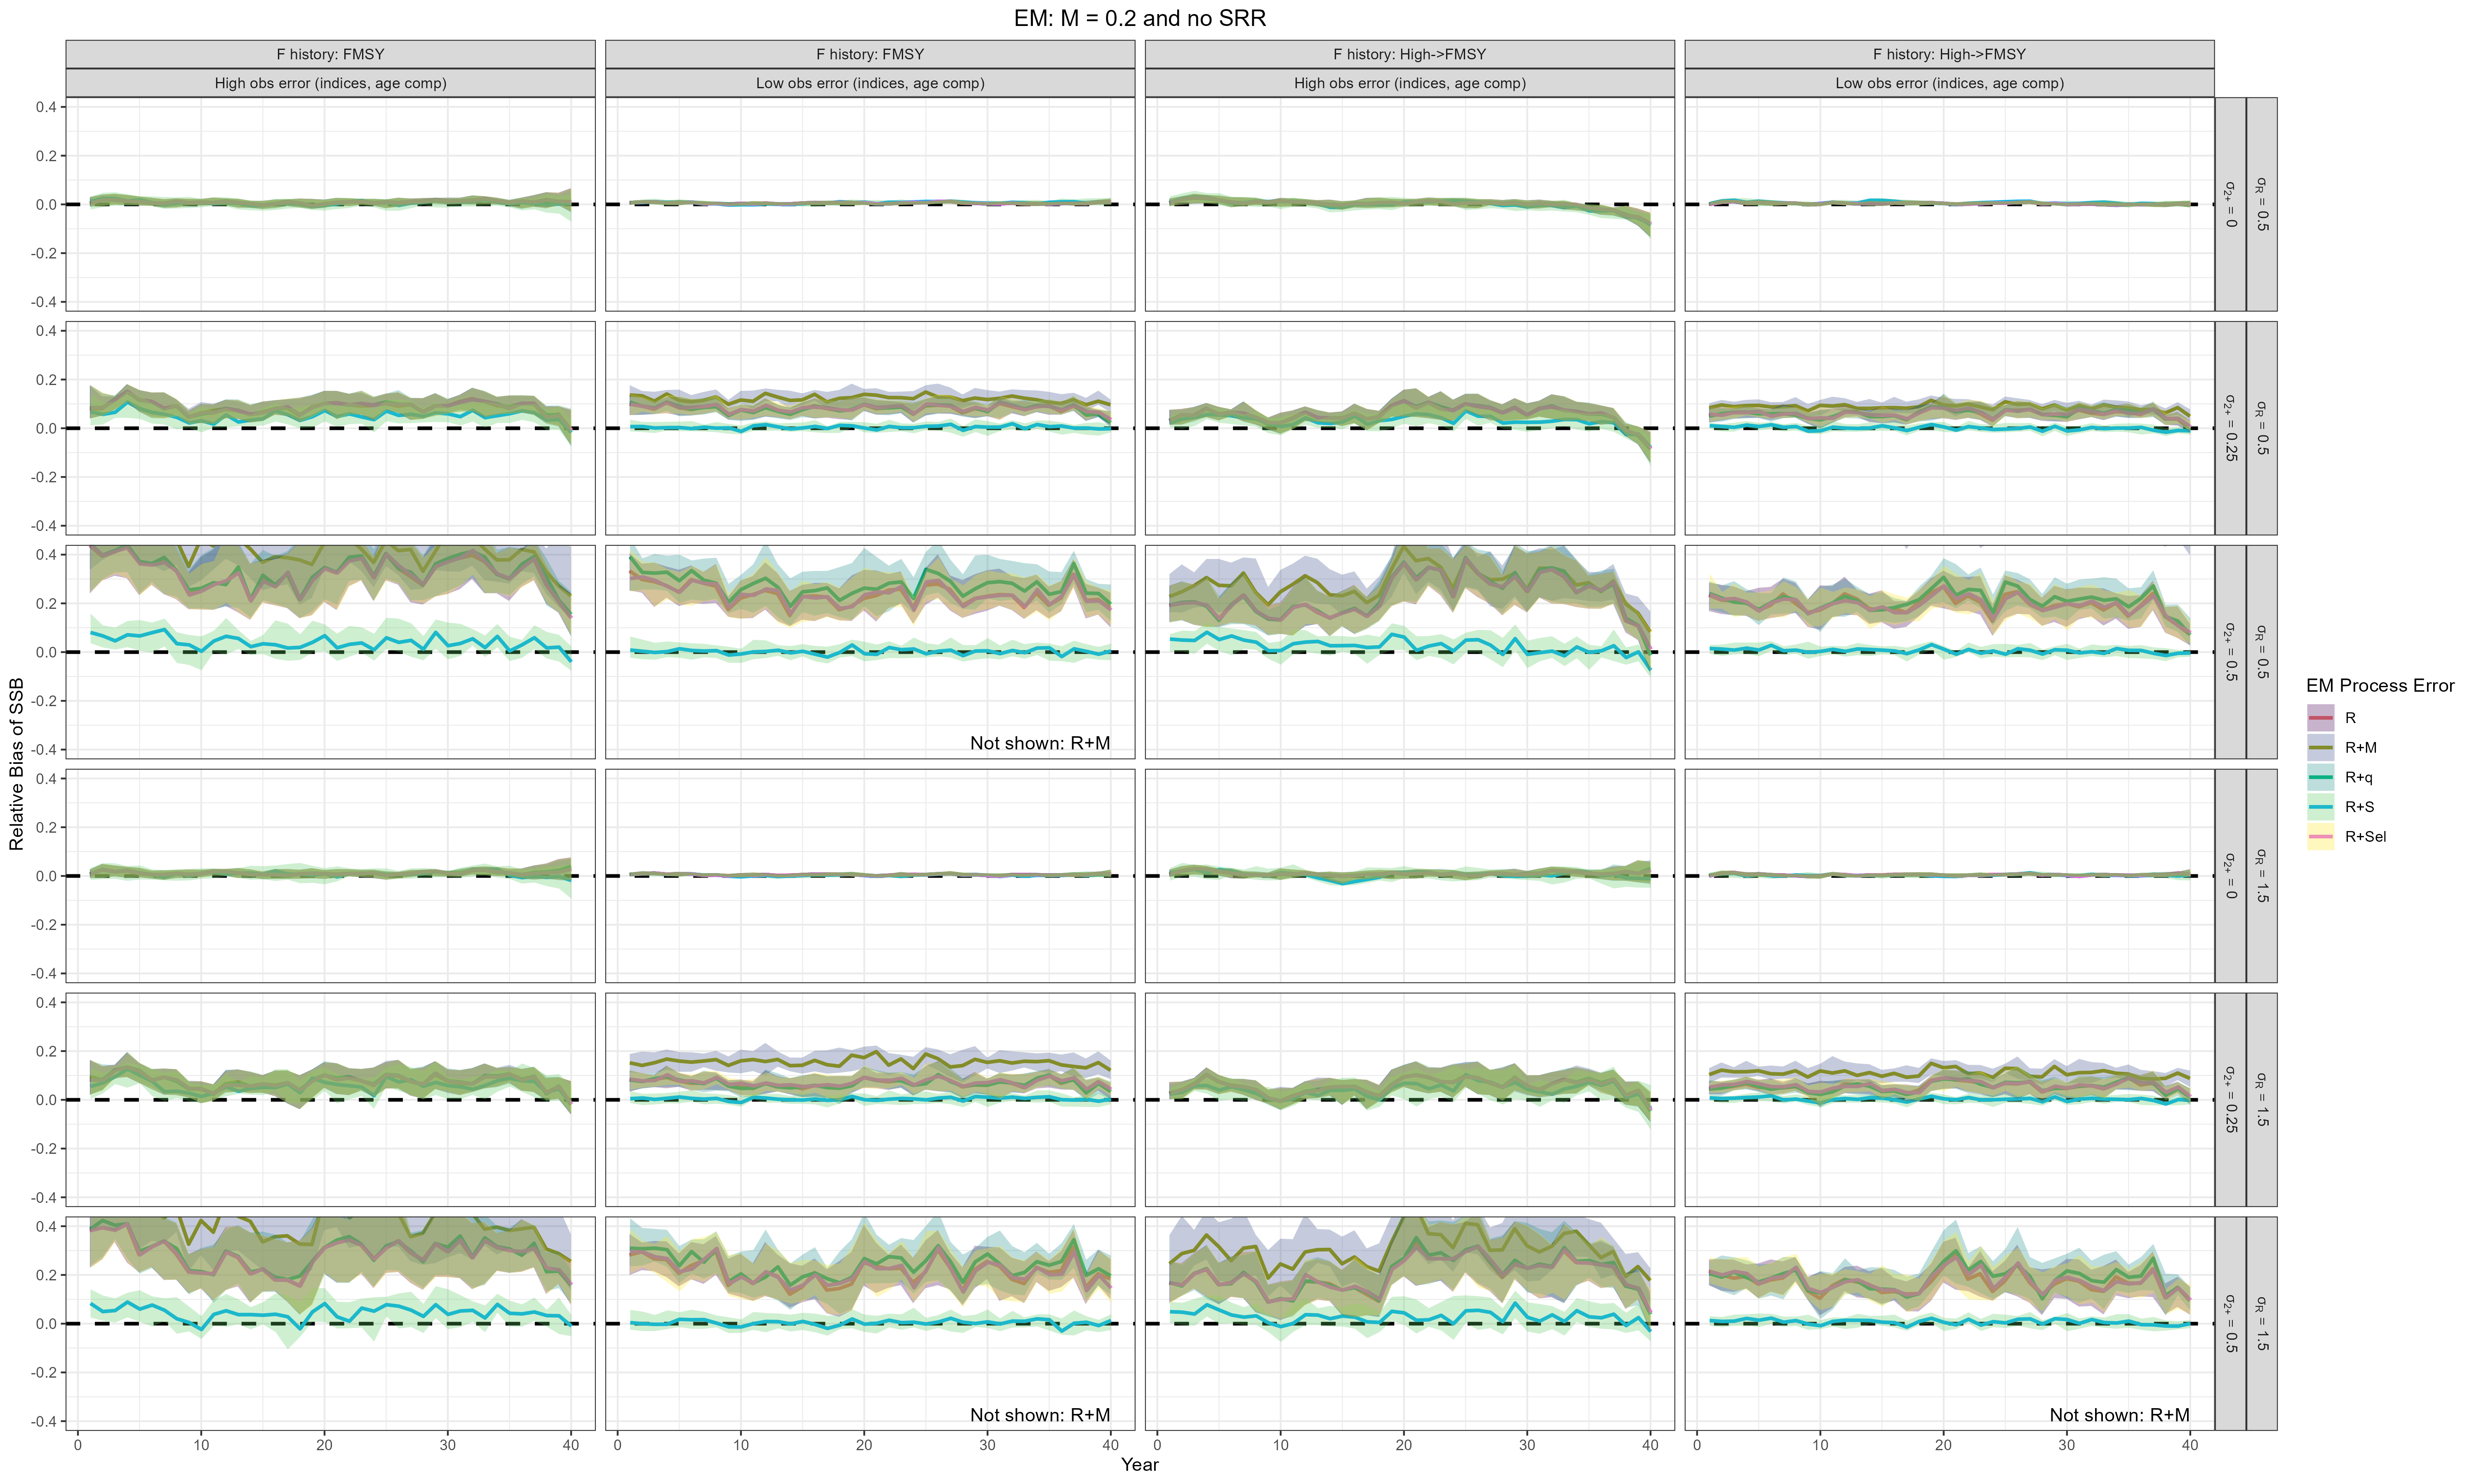
\includegraphics[width = \textwidth]{naa_om_R_MF_relbias_ssb.png}
\end{center}
\end{figure}
\end{landscape}

\begin{landscape}
\begin{figure}
\caption{Median relative bias of for SSB for estimating models that estimate mean recruitment and M is estimated.}\label{naa_om_em_R_ME_relbias_ssb}
\begin{center}
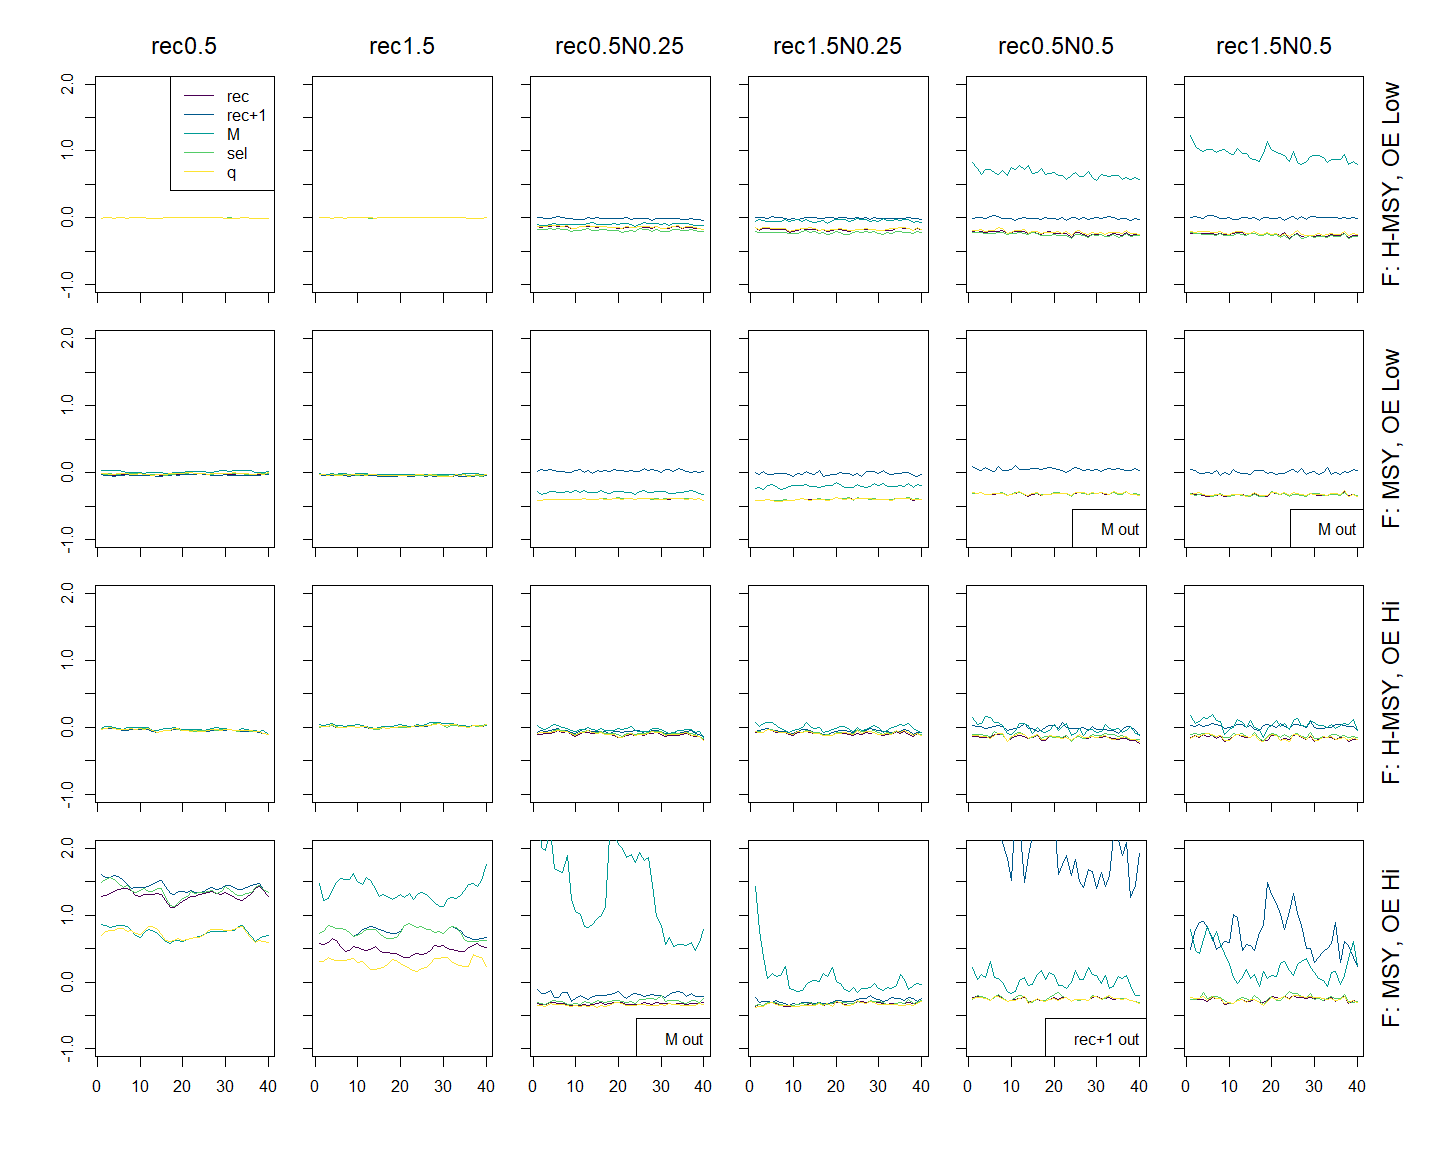
\includegraphics[width = \textwidth]{naa_om_R_ME_relbias_ssb.png}
\end{center}
\end{figure}
\end{landscape}

\begin{landscape}
\begin{figure}
\caption{Median relative bias of for SSB for estimating models that estimates a BH stock-recruitment function and M is fixed at the true value.}\label{naa_om_em_SR_MF_relbias_ssb}
\begin{center}
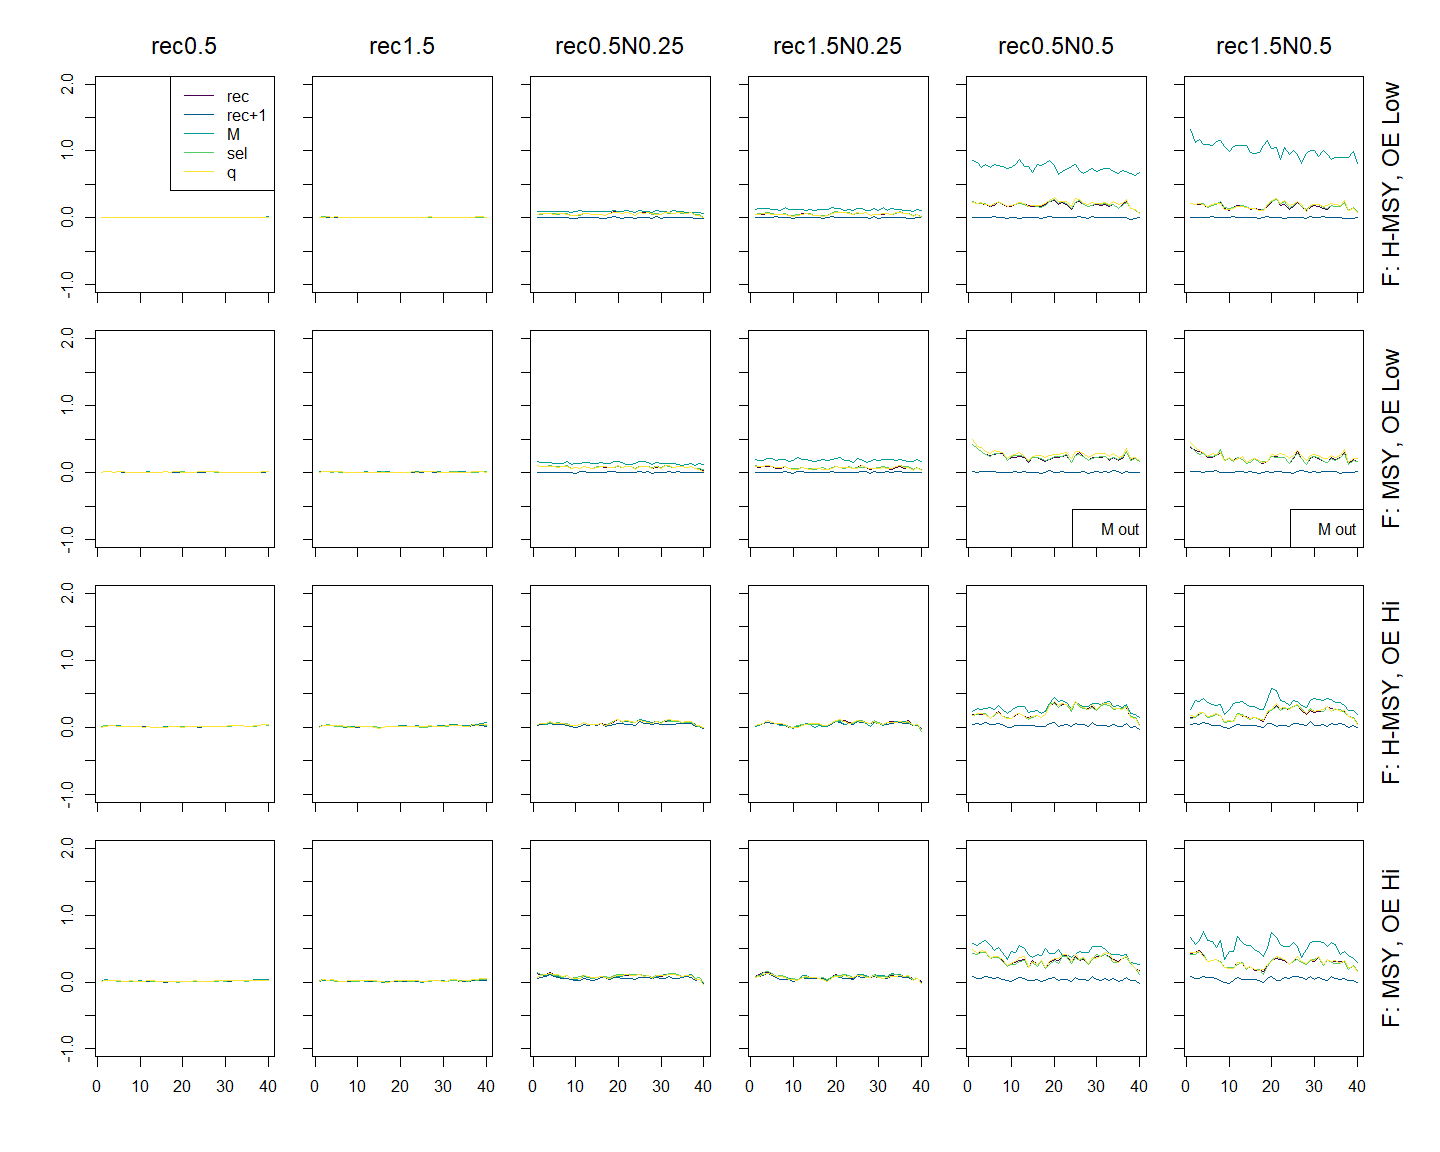
\includegraphics[width = \textwidth]{naa_om_SR_MF_relbias_ssb.png}
\end{center}
\end{figure}
\end{landscape}

\begin{landscape}
\begin{figure}
\caption{Median relative bias of for SSB for estimating models that estimates a BH stock-recruitment function and M is estimated.}\label{naa_om_em_SR_ME_relbias_ssb}
\begin{center}
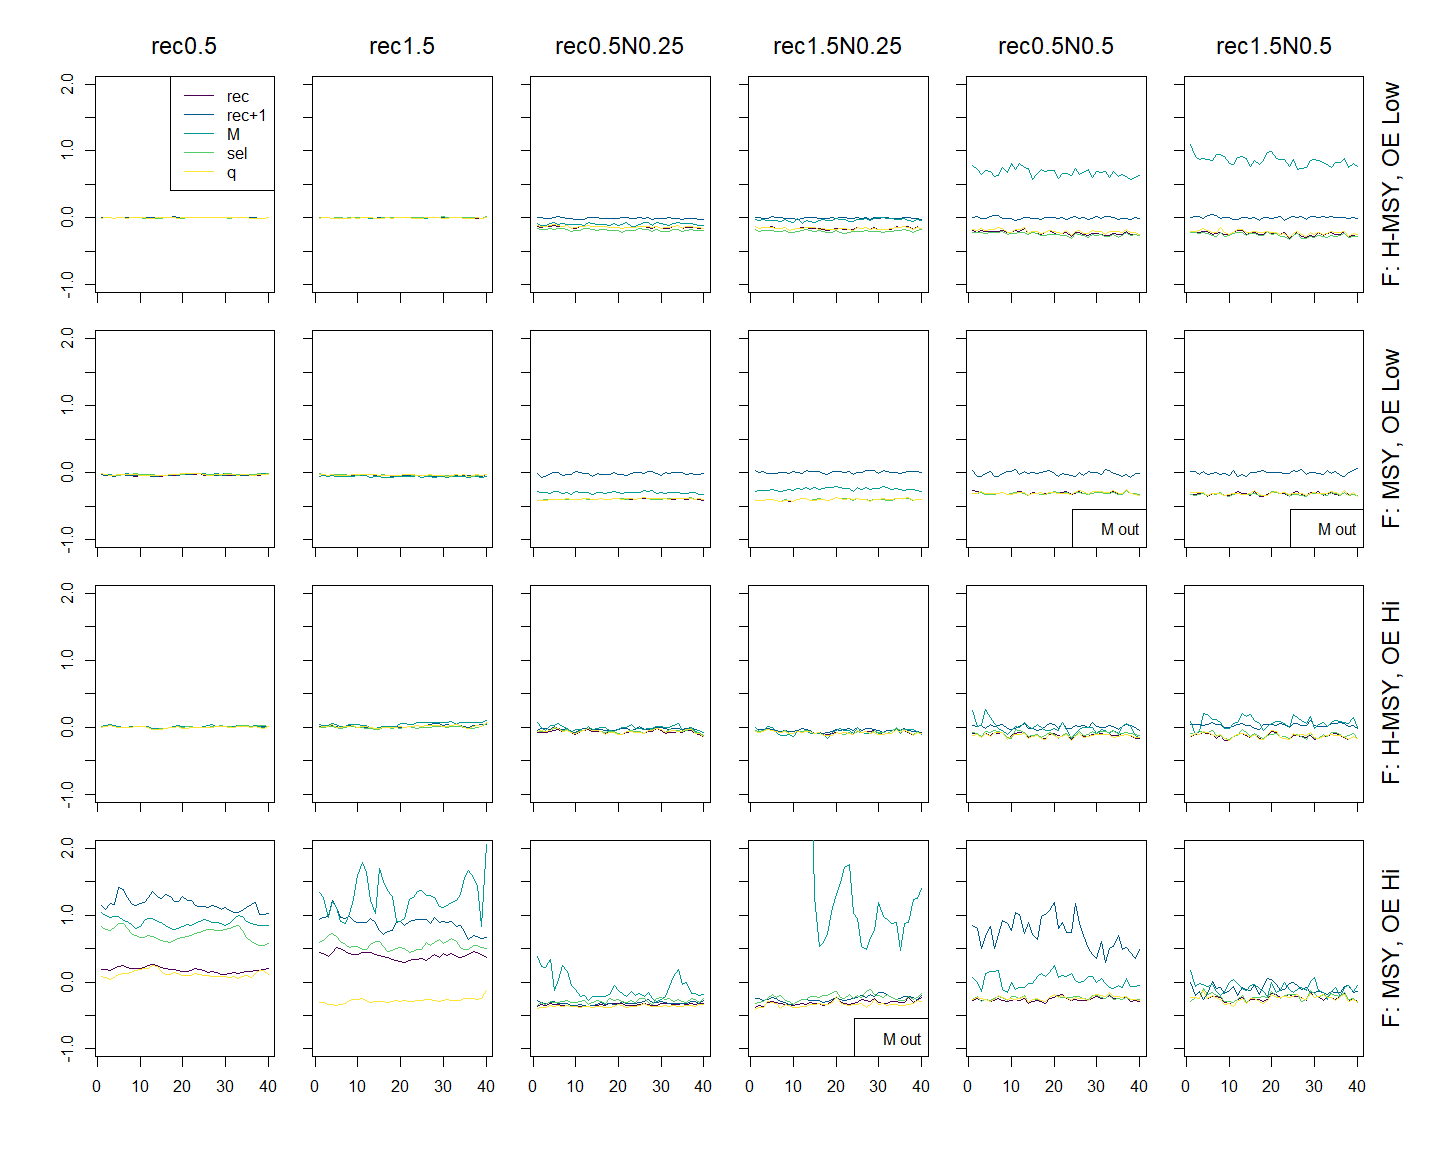
\includegraphics[width = \textwidth]{naa_om_SR_ME_relbias_ssb.png}
\end{center}
\end{figure}
\end{landscape}

\hypertarget{estimating-models-include-naa-random-effects-and-estimation-assumes-mean-r-or-bh-sr}{%
\subsubsection{Estimating models include NAA random effects and
estimation assumes mean R or BH
SR}\label{estimating-models-include-naa-random-effects-and-estimation-assumes-mean-r-or-bh-sr}}

\clearpage

\begin{table}
\caption{Operating models and estimation models all assume RE on recruitment only, estimating models assume mean recruitment or a B-H stock recruit relationship and M is fixed at the true value.}
{%latex.default(out, file = here("Project_0", "paper", "rec_om_em_R_SR_MF_aic_table.tex"),     table.env = FALSE, col.just = rep("r", dim(out)[2]), rowname = NULL)%
\begin{center}
\begin{tabular}{rrrrrr}
\hline\hline
\multicolumn{1}{c}{$\sigma_R$}&\multicolumn{1}{c}{$\sigma_N$}&\multicolumn{1}{c}{F-history}&\multicolumn{1}{c}{Obs Error}&\multicolumn{1}{c}{R only}&\multicolumn{1}{c}{BH}\tabularnewline
\hline
$0.5$&$$&H-MSY&L&$46$&$54$\tabularnewline
$1.5$&$$&H-MSY&L&$82$&$18$\tabularnewline
$0.5$&$$&MSY&L&$71$&$29$\tabularnewline
$1.5$&$$&MSY&L&$85$&$15$\tabularnewline
$0.5$&$$&H-MSY&H&$51$&$49$\tabularnewline
$1.5$&$$&H-MSY&H&$82$&$18$\tabularnewline
$0.5$&$$&MSY&H&$72$&$28$\tabularnewline
$1.5$&$$&MSY&H&$86$&$14$\tabularnewline
\hline
\end{tabular}\end{center}
}
\end{table}

\begin{table}
\caption{Operating models and estimation models all assume RE on recruitment only, estimating models assume mean recruitment or a B-H stock recruit relationship and M is estimated.}
{%latex.default(out, file = here("Project_0", "paper", "rec_om_em_R_SR_ME_aic_table.tex"),     table.env = FALSE, col.just = rep("r", dim(out)[2]), rowname = NULL)%
\begin{center}
\begin{tabular}{rrrrrr}
\hline\hline
\multicolumn{1}{c}{$\sigma_R$}&\multicolumn{1}{c}{$\sigma_N$}&\multicolumn{1}{c}{F-history}&\multicolumn{1}{c}{Obs Error}&\multicolumn{1}{c}{R only}&\multicolumn{1}{c}{BH}\tabularnewline
\hline
$0.5$&$$&H-MSY&L&$45$&$55$\tabularnewline
$1.5$&$$&H-MSY&L&$82$&$18$\tabularnewline
$0.5$&$$&MSY&L&$70$&$30$\tabularnewline
$1.5$&$$&MSY&L&$87$&$13$\tabularnewline
$0.5$&$$&H-MSY&H&$56$&$44$\tabularnewline
$1.5$&$$&H-MSY&H&$82$&$18$\tabularnewline
$0.5$&$$&MSY&H&$75$&$25$\tabularnewline
$1.5$&$$&MSY&H&$84$&$16$\tabularnewline
\hline
\end{tabular}\end{center}
}
\end{table}

\begin{table}
\caption{Operating models and estimation models all assume RE on all abundances at age, estimating models assume mean recruitment or a B-H stock recruit relationship and M is fixed at the true value.}
{%latex.default(out, file = here("Project_0", "paper", "naa_om_em_R_SR_MF_aic_table.tex"),     table.env = FALSE, col.just = rep("r", dim(out)[2]), rowname = NULL)%
\begin{center}
\begin{tabular}{rrrrrr}
\hline\hline
\multicolumn{1}{c}{$\sigma_R$}&\multicolumn{1}{c}{$\sigma_N$}&\multicolumn{1}{c}{F-history}&\multicolumn{1}{c}{Obs Error}&\multicolumn{1}{c}{R only}&\multicolumn{1}{c}{BH}\tabularnewline
\hline
$0.5$&$0.25$&H-MSY&L&$43$&$57$\tabularnewline
$1.5$&$0.25$&H-MSY&L&$84$&$16$\tabularnewline
$0.5$&$0.50$&H-MSY&L&$33$&$67$\tabularnewline
$1.5$&$0.50$&H-MSY&L&$77$&$23$\tabularnewline
$0.5$&$0.25$&MSY&L&$69$&$31$\tabularnewline
$1.5$&$0.25$&MSY&L&$88$&$12$\tabularnewline
$0.5$&$0.50$&MSY&L&$55$&$45$\tabularnewline
$1.5$&$0.50$&MSY&L&$87$&$13$\tabularnewline
$0.5$&$0.25$&H-MSY&H&$57$&$43$\tabularnewline
$1.5$&$0.25$&H-MSY&H&$84$&$16$\tabularnewline
$0.5$&$0.50$&H-MSY&H&$66$&$34$\tabularnewline
$1.5$&$0.50$&H-MSY&H&$79$&$21$\tabularnewline
$0.5$&$0.25$&MSY&H&$78$&$22$\tabularnewline
$1.5$&$0.25$&MSY&H&$88$&$12$\tabularnewline
$0.5$&$0.50$&MSY&H&$73$&$27$\tabularnewline
$1.5$&$0.50$&MSY&H&$83$&$17$\tabularnewline
\hline
\end{tabular}\end{center}
}
\end{table}

\begin{table}
\caption{Operating models and estimation models all assume RE on all abundances at age, estimating models assume mean recruitment or a B-H stock recruit relationship and M is estimated.}
{%latex.default(out, file = here("Project_0", "paper", "naa_om_em_R_SR_ME_aic_table.tex"),     table.env = FALSE, col.just = rep("r", dim(out)[2]), rowname = NULL)%
\begin{center}
\begin{tabular}{rrrrrr}
\hline\hline
\multicolumn{1}{c}{$\sigma_R$}&\multicolumn{1}{c}{$\sigma_N$}&\multicolumn{1}{c}{F-history}&\multicolumn{1}{c}{Obs Error}&\multicolumn{1}{c}{R only}&\multicolumn{1}{c}{BH}\tabularnewline
\hline
$0.5$&$0.25$&H-MSY&L&$44$&$56$\tabularnewline
$1.5$&$0.25$&H-MSY&L&$84$&$16$\tabularnewline
$0.5$&$0.50$&H-MSY&L&$31$&$69$\tabularnewline
$1.5$&$0.50$&H-MSY&L&$80$&$20$\tabularnewline
$0.5$&$0.25$&MSY&L&$68$&$32$\tabularnewline
$1.5$&$0.25$&MSY&L&$88$&$12$\tabularnewline
$0.5$&$0.50$&MSY&L&$55$&$45$\tabularnewline
$1.5$&$0.50$&MSY&L&$86$&$14$\tabularnewline
$0.5$&$0.25$&H-MSY&H&$59$&$41$\tabularnewline
$1.5$&$0.25$&H-MSY&H&$81$&$19$\tabularnewline
$0.5$&$0.50$&H-MSY&H&$67$&$33$\tabularnewline
$1.5$&$0.50$&H-MSY&H&$80$&$20$\tabularnewline
$0.5$&$0.25$&MSY&H&$66$&$34$\tabularnewline
$1.5$&$0.25$&MSY&H&$74$&$26$\tabularnewline
$0.5$&$0.50$&MSY&H&$74$&$26$\tabularnewline
$1.5$&$0.50$&MSY&H&$87$&$13$\tabularnewline
\hline
\end{tabular}\end{center}
}
\end{table}
\clearpage

\begin{figure}
\caption{Predicted probability of AIC being better for BH model.}\label{glm_res_NAA_re}
\begin{center}
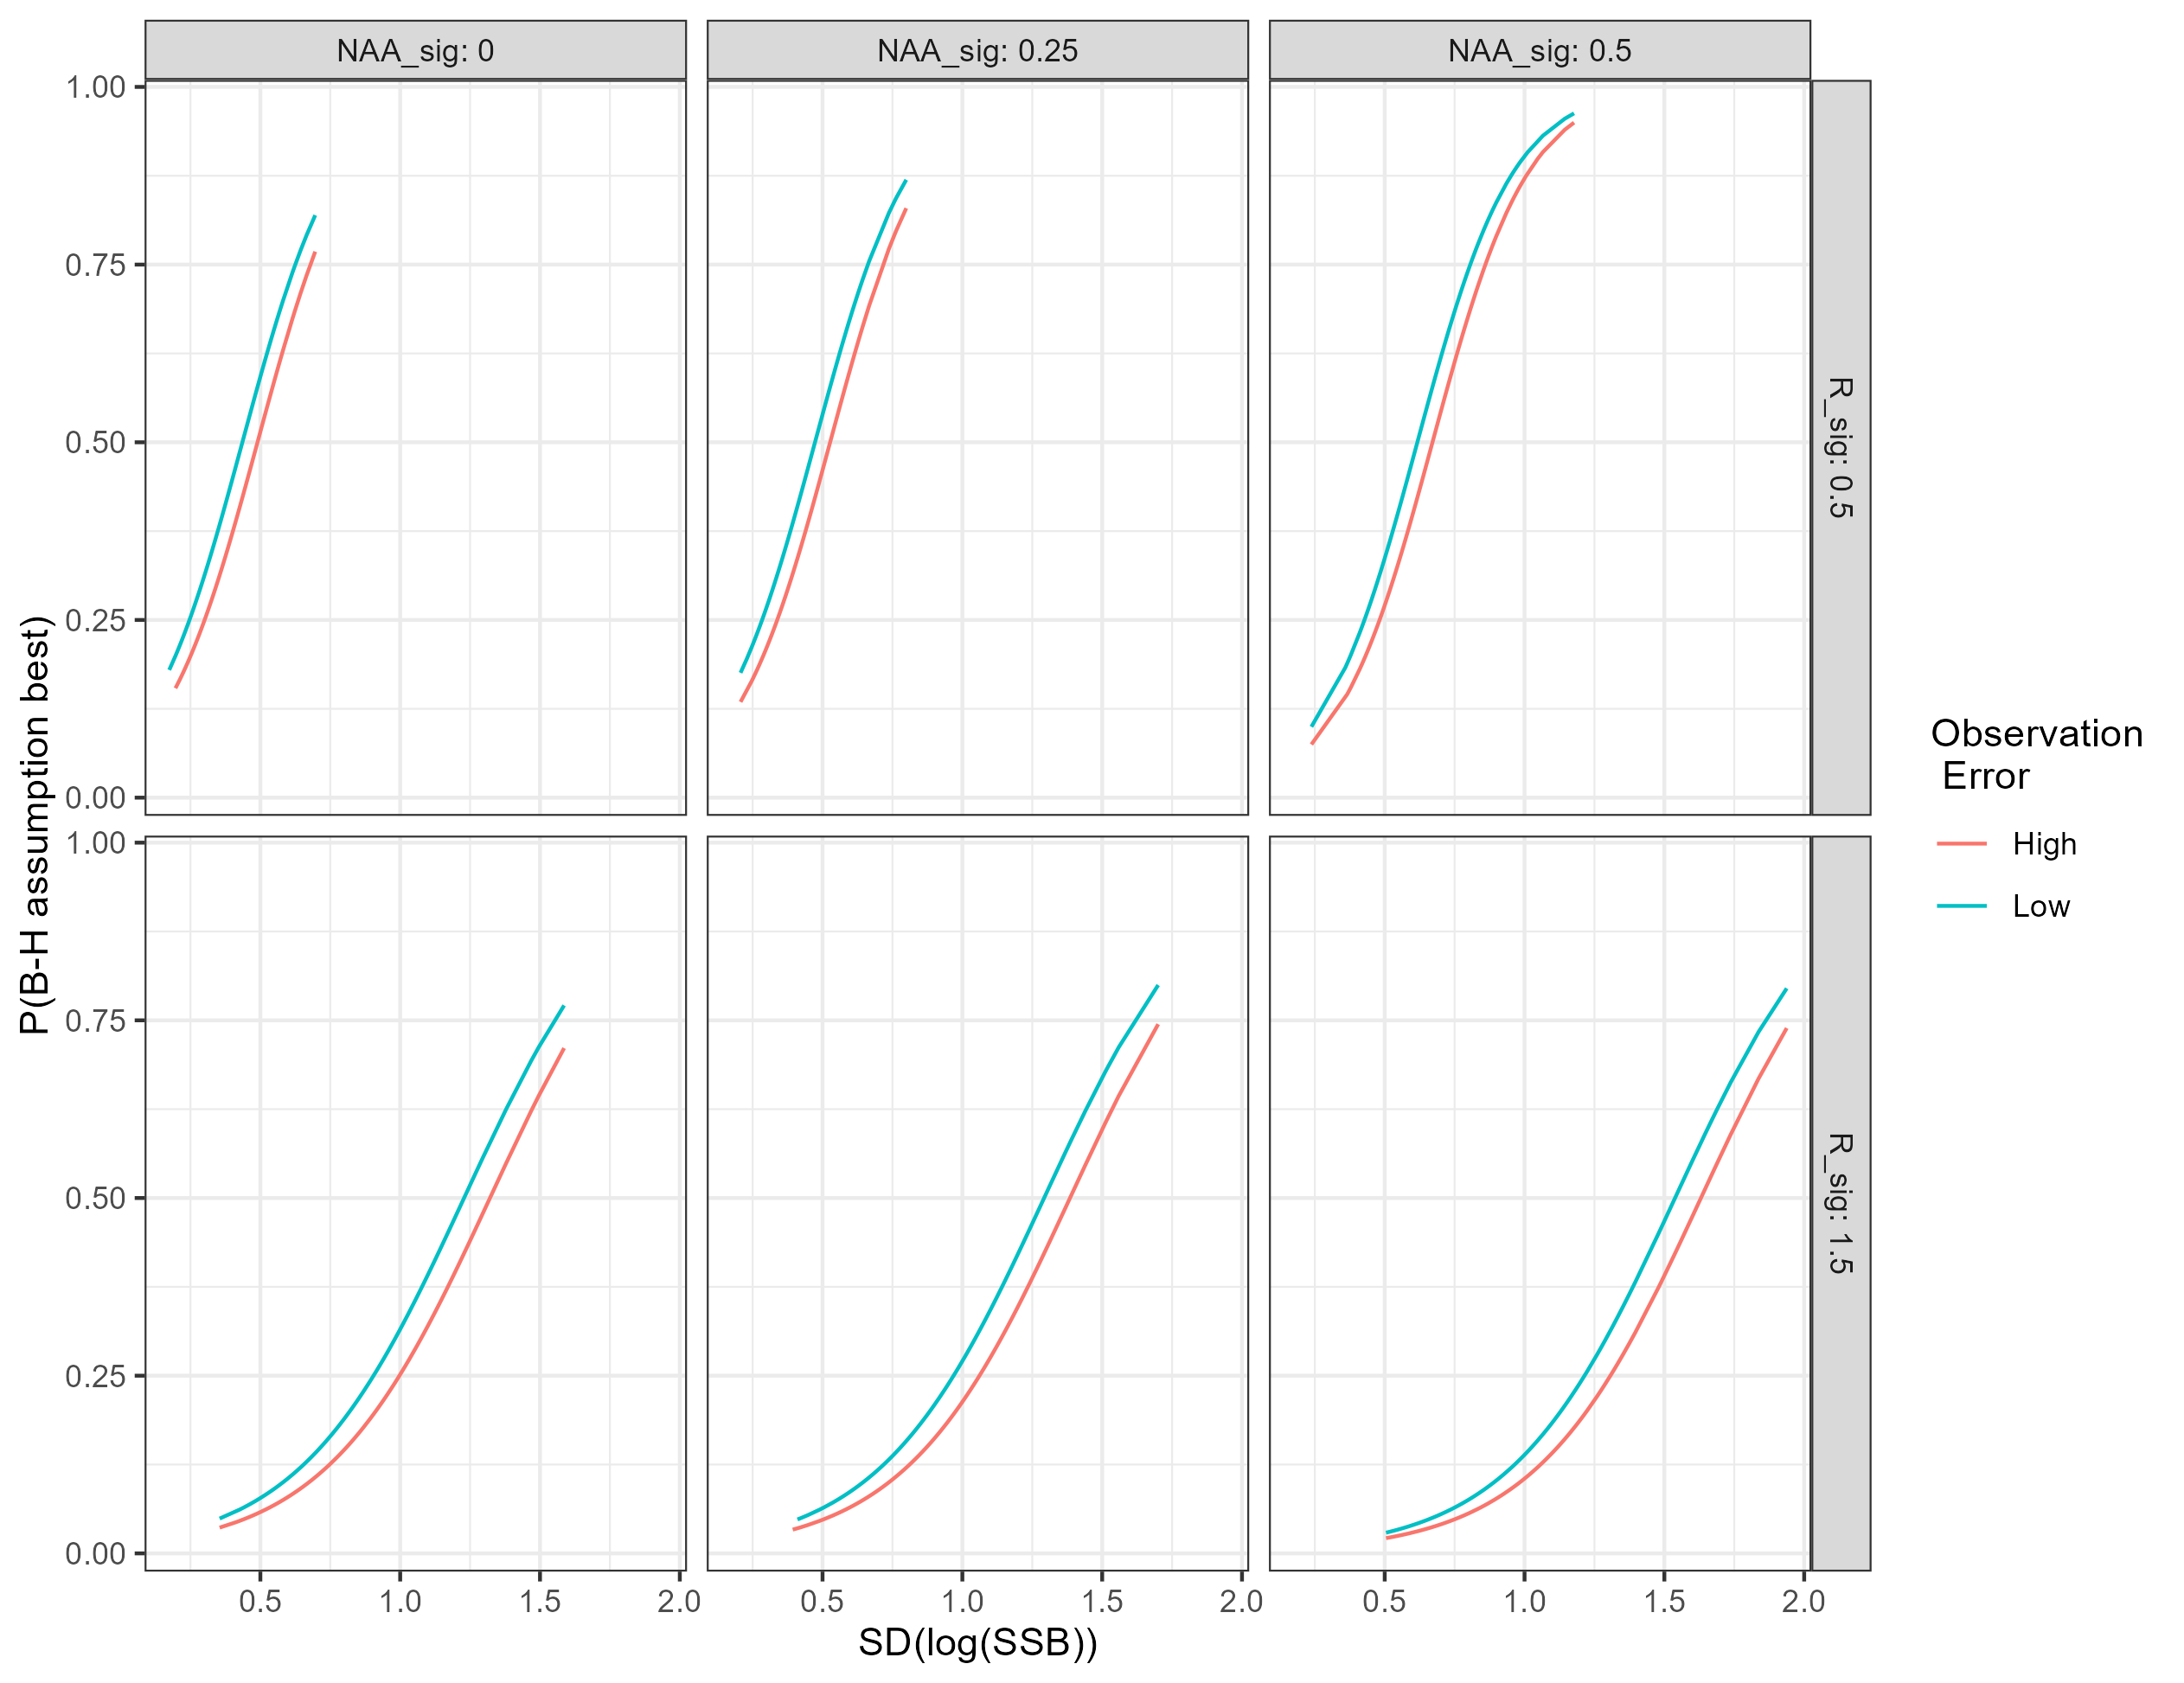
\includegraphics[width = \textwidth]{pred_SR_best_NAA_oms.png}
\end{center}
\end{figure}

\hypertarget{m-operating-models}{%
\subsection{M operating models}\label{m-operating-models}}

\hypertarget{estimating-models-include-naa-random-effects-and-estimation-assumes-mean-r-or-bh-sr-1}{%
\subsubsection{Estimating models include NAA random effects and
estimation assumes mean R or BH
SR}\label{estimating-models-include-naa-random-effects-and-estimation-assumes-mean-r-or-bh-sr-1}}

\begin{table}
\caption{M random effects operating models.}
{%latex.default(out, file = here("Project_0", "paper", "M_om_em_R_BH_aic_table.tex"),     table.env = FALSE, col.just = rep("r", dim(out)[2]), rowname = NULL)%
\begin{center}
\begin{tabular}{rrrrrrrr}
\hline\hline
\multicolumn{1}{c}{$\sigma_M$}&\multicolumn{1}{c}{$\rho_M$}&\multicolumn{1}{c}{F-history}&\multicolumn{1}{c}{Obs Error}&\multicolumn{1}{c}{R (M fix)}&\multicolumn{1}{c}{BH (M fix)}&\multicolumn{1}{c}{R (M est)}&\multicolumn{1}{c}{BH (M est)}\tabularnewline
\hline
$0.1$&$0.0$&H-MSY&L&$38$&$62$&$38$&$62$\tabularnewline
$0.5$&$0.0$&H-MSY&L&$42$&$58$&$42$&$58$\tabularnewline
$0.1$&$0.0$&MSY&L&$66$&$34$&$66$&$34$\tabularnewline
$0.5$&$0.0$&MSY&L&$70$&$30$&$58$&$41$\tabularnewline
$0.1$&$0.0$&H-MSY&H&$45$&$55$&$47$&$53$\tabularnewline
$0.5$&$0.0$&H-MSY&H&$56$&$43$&$54$&$45$\tabularnewline
$0.1$&$0.0$&MSY&H&$66$&$34$&$66$&$33$\tabularnewline
$0.5$&$0.0$&MSY&H&$72$&$28$&$57$&$42$\tabularnewline
$0.1$&$0.9$&H-MSY&L&$31$&$69$&$33$&$64$\tabularnewline
$0.5$&$0.9$&H-MSY&L&$15$&$73$&$16$&$64$\tabularnewline
$0.1$&$0.9$&MSY&L&$44$&$56$&$41$&$47$\tabularnewline
$0.5$&$0.9$&MSY&L&$12$&$76$&$10$&$69$\tabularnewline
$0.1$&$0.9$&H-MSY&H&$32$&$68$&$47$&$44$\tabularnewline
$0.5$&$0.9$&H-MSY&H&$10$&$78$&$21$&$51$\tabularnewline
$0.1$&$0.9$&MSY&H&$40$&$60$&$38$&$28$\tabularnewline
$0.5$&$0.9$&MSY&H&$22$&$64$&$22$&$49$\tabularnewline
\hline
\end{tabular}\end{center}
}
\end{table}
\clearpage

\hypertarget{discussion}{%
\section{Discussion}\label{discussion}}

The estimating models assumed variances of aggregate catch and index
observations was known. This approximation may be appropriate for
indices where we have a reliable estimate of uncertainty based on the
survey design (), but there may be better approaches for the aggregate
catch such as an informed prior on the standard errors with realistic
bounds.

\hypertarget{acknowledgements}{%
\section*{Acknowledgements}\label{acknowledgements}}
\addcontentsline{toc}{section}{Acknowledgements}

This work was funded by NOAA Fisheries Northeast Fisheries Science
Center.

\pagebreak

\bibliography{paper}

\hypertarget{refs}{}
\begin{CSLReferences}{0}{0}
\end{CSLReferences}

\pagebreak

\clearpage

\end{document}
